\documentclass{cccg20}
\usepackage{graphicx,amssymb,amsmath}
\usepackage[hyphens]{url}
\usepackage{booktabs}

%----------------------- Macros and Definitions --------------------------
\fancyhead{}
\fancyhead[RO]{\sf COMP 4801 Project Report, Fall 2026}
\fancyhead[LE]{\sf Cardinality Sketches under Adaptive Inputs}

\newcommand{\E}{\mathbb{E}}
\newcommand{\Var}{\mathrm{Var}}
\newcommand{\Exp}{\mathrm{Exp}}
\newcommand{\est}{\mathcal{M}}
\newtheorem{definition}{Definition}

%----------------------- Title -------------------------------------------
\title{Cardinality Sketches under Adaptive Inputs:\\ A Study and Replication of a Linear-Size Attack}
\author{Ryan Zhu\\ {\small Student no.\ 101301524}}

\begin{document}
\thispagestyle{empty}
\maketitle

\begin{abstract}
Cardinality sketches such as bottom-$k$ and HyperLogLog (HLL) summarize a set in $O(k)$ space, can be merged, and estimate the number of distinct keys with relative error about $1/\sqrt{k}$. That guarantee silently assumes each query is independent of the sketch's hash randomness. We study the recent work of Ahmadian and Cohen~\cite{ahmadian2024}, which shows that queries that adapt to earlier answers break this assumption: a single batch of $O(k)$ random queries, plus simple post-processing, yields a set whose estimate is far off, and $\tilde O(k^2)$ adaptive queries defeat \emph{any} estimator. We explain why the non-adaptive guarantee fails, sketch the analysis of the linear attack, and implement it. Our experiments reproduce the paper's headline result on HLL and extend it to bottom-$k$, the sketch the theorem is actually proved for: with $r=4k$ queries, for every $k$ from 64 to 2048, we construct sets that HLL overestimates by $2.0$--$2.7\times$ (mean $2.3\times$; bottom-$k$: $3.8$--$5.6\times$, mean $4.7\times$) and underestimates by about half. Re-drawing the hash randomness every $B\le k/2$ queries stops the attack, but at the cost of mergeability.
\end{abstract}

%=========================================================================
\section{Introduction}

\paragraph{Motivation.}
Counting distinct elements is a basic primitive in databases, network monitoring, and analytics. Exact counting needs space linear in the number of distinct keys, so systems such as Google BigQuery and Apache DataSketches use \emph{cardinality sketches}~\cite{flajolet1985,cohen1997,flajolet2007,heule2013}. A sketch $S_\rho(U)$ of a set $U$ is computed with internal randomness $\rho$ (hash functions), uses $O(k)$ registers, and supports an estimator $\est$ with normalized root mean squared error (NRMSE) about $1/\sqrt{k}$. Crucially, sketches are \emph{composable}: $S_\rho(U\cup V)$ can be computed from $S_\rho(U)$ and $S_\rho(V)$. This is what makes them useful in distributed and streaming settings, but it only works if every sketch in the system uses the \emph{same} $\rho$. The randomness is therefore fixed once and reused for every query.

\paragraph{The hidden assumption.}
In class we saw that the textbook $p^k$ false-positive bound for Bloom filters is wrong because the $k$ probed bits all read one shared random array and are not independent~\cite{bose2008}. Cardinality sketches have an analogous hidden assumption: every accuracy guarantee is for a query set $U$ chosen \emph{independently} of $\rho$. This is the oblivious-versus-adaptive adversary distinction from the multiplicative weights unit. If the queries are fixed in advance, a union bound shows that exponentially many of them are answered correctly. But if the next query may depend on earlier answers, information about $\rho$ leaks and the union bound no longer applies.

\paragraph{Problem statement.}
We study three questions raised by~\cite{ahmadian2024}: (1) why the union bound gives exponentially many safe non-adaptive queries and why it fails for adaptive ones; (2) how averaging the responses to $O(k)$ random subset queries reveals the lowest-hash keys and yields an adversarial set (their Algorithm~1 and Theorem~4.1); and (3) why any correct estimator can be defeated with roughly $k^2$ adaptive queries, and why such an attack needs several rounds.

\paragraph{Related work.}
Hardt and Woodruff~\cite{hardt2013} showed that linear sketches cannot be robust to adaptive inputs in general. Ben-Eliezer et al.~\cite{beneliezer2020} gave generic frameworks that make streaming algorithms robust at a cost in space, and Hassidim et al.~\cite{hassidim2020} used differential privacy to support $r^2$ adaptive queries with $\tilde O(r)$ sketches, which is tight for generic methods. Reviriego and Ting~\cite{reviriego2020} gave streaming attacks on HLL that detect, one insertion at a time, which keys change the estimate. The attacks of~\cite{ahmadian2024} are stronger: the linear attack is a single batch of non-adaptive queries, and only the post-processing is adaptive.

\paragraph{What we did.}
We implemented bottom-$k$ and HLL sketches and Algorithm~1 of~\cite{ahmadian2024} in Python. We confirmed the $1/\sqrt{k}$ error for non-adaptive queries, reproduced the attack curves of the paper as a function of the number of queries $r$ and the sketch size $k$, and ran the same attack on bottom-$k$, for which Theorem~4.1 is proved but which the paper does not test empirically. We also measured a simple mitigation that re-draws the hash randomness every $B$ queries.

%=========================================================================
\section{Preliminaries}

Let $\mathcal U$ be a universe of keys. All sketches below assign each key random ``priorities'' with hash functions and keep the lowest priorities seen in $U$; a larger set tends to contain smaller priorities.

\paragraph{MinHash sketches~\cite{ahmadian2024}.}
\emph{$k$-mins} uses $k$ hash functions $h_i:\mathcal U\to\Exp[1]$ and stores $(\min_{x\in U} h_i(x))_{i\in[k]}$, i.e.\ $k$ i.i.d.\ $\Exp[|U|]$ values; with $T(S)=\sum_i S_i$ the estimate is $(k-1)/T$.
\emph{Bottom-$k$} uses one hash $h:\mathcal U\to U[0,1]$ and stores the $k$ smallest values of $h$ on $U$; with $T(S)$ the $k$-th smallest, the estimate is $(k-1)/T$.
\emph{$k$-partition} splits keys into $k$ buckets by a hash and keeps the minimum of $h$ in each.
\emph{HyperLogLog}~\cite{flajolet2007} is a discretized $k$-partition sketch: each of $k=2^p$ registers stores the maximum, over keys in its bucket, of the position of the leading one-bit of the hash (a rounded $-\log_2$ of the minimum), and the estimate is $\alpha_k k^2/\sum_j 2^{-M_j}$ (linear counting for small sets; HLL++~\cite{heule2013} adds a sparse mode and small-range bias correction).
All have NRMSE $\approx 1/\sqrt{k}$ ($1.04/\sqrt{k}$ for HLL).

A statistic $T$ of the sketch is \emph{sufficient} if it carries all the information the sketch has about $|U|$. The ``standard'' estimators report a function of a sufficient statistic. Following~\cite{ahmadian2024}, a set $U$ is \emph{adversarial} for $\rho$ if $T(S_\rho(U))$ is far in the tail of its distribution under random $\rho$; e.g.\ the sketch is \emph{biased up by $1/\alpha$} if $T(S_\rho(U))\le \alpha k/|U|$, which for $\alpha\le 1/2$ has probability $e^{-\Omega(k)}$ under random $\rho$.

\paragraph{The non-adaptive guarantee (Problem 1).}
A sketch with $k=O(\epsilon^{-2}\log(1/\delta))$ satisfies, for every \emph{fixed} $U$,
$\Pr_\rho\bigl[|\est(S_\rho(U))-|U||>\epsilon|U|\bigr]\le\delta$,
so $\delta=e^{-\Omega(\epsilon^2 k)}$. If the $r$ query sets $U_1,\dots,U_r$ are fixed before $\rho$ is drawn, a union bound over these $r$ events shows that all $r$ answers are within $1\pm\epsilon$ with probability $\ge 1-r\delta$. Hence a sketch of size $k$ answers $r=e^{\Omega(\epsilon^2 k)}$ non-adaptive queries correctly: exponentially many in $k$.

The argument breaks once $U_{i}$ may depend on the answers to $U_1,\dots,U_{i-1}$. Each answer is a function of $\rho$, so $U_{i}$ becomes a random variable correlated with $\rho$. The event ``the answer on $U_i$ is bad'' is no longer the event for a fixed set, and the union bound would have to range over every set the adversary might choose. If queries are drawn from a pool of $n$ keys, that is $2^n$ sets, and $2^n\delta\gg 1$ is useless. Concretely, every answer leaks a little about which keys have low priority, and since $\rho$ is reused, this information accumulates. This is the same failure as in the Bloom filter analysis: an argument that treats as independent things that share one random object.

%=========================================================================
\section{Attacks on Cardinality Sketches}

\subsection{Single-batch attack on standard estimators (Problem 2)}

\begin{figure}[t]
\centering
\fbox{\parbox{0.94\columnwidth}{\small
\textbf{Algorithm 1} (attack on standard estimators~\cite{ahmadian2024})\\[2pt]
\textbf{Input:} query access to $\est(S_\rho(\cdot))$; ground set $N$ of $n$ keys chosen independently of $\rho$; number of queries $r$.\\[2pt]
1.\ For all $x\in N$: $c[x]\gets 0$, $t[x]\gets 0$.\\
2.\ \textbf{for} $i=1,\dots,r$ \textbf{do}\\
\hspace*{1.2em}$U\gets$ each $x\in N$ independently w.p.\ $1/2$\\
\hspace*{1.2em}$T\gets 1/\est(S_\rho(U))$ \hfill\emph{(one query)}\\
\hspace*{1.2em}for all $x\in U$: $t[x]\gets t[x]+1$, $c[x]\gets c[x]+T$\\
3.\ \textbf{return} keys of $N$ sorted by $A[x]=c[x]/t[x]$.\\[2pt]
A prefix of the order is overestimated; a suffix is underestimated.
}}
\end{figure}

The attack (Algorithm~1) fixes a ground set $N$ of $n\gg k$ keys and asks $r$ queries, each a uniformly random half of $N$. All queries are drawn from the same distribution before any answer is seen, so it is a single batch: the only adaptive step is the post-processing. For each key $x$ the attacker records the average $A[x]$ of the statistic $T=1/\est$ over the queries that contained $x$.

\paragraph{Why it works.}
A key that is one of the lowest-priority keys of $N$ (one that sets a sketch register whenever it is present) makes the sketch look larger whenever it is in $U$, so $T$ is smaller on those queries. A ``transparent'' key, one with high priority, almost never affects the sketch, and its average $A[x]$ is just the overall mean of $T$. So low-priority keys get systematically \emph{lower} average scores. Sorting by $A$ puts them first. The prefix $U_\alpha$ of the $\alpha n$ lowest-score keys then contains most of the $O(k)$ keys that determine $S_\rho(N)$. Its sketch looks almost like the sketch of all of $N$, so its estimate is close to $n$ instead of $\alpha n$. Symmetrically, the highest-score keys avoid the low-priority keys and their sketch looks too small.

\begin{theorem}[Theorem 4.1 of~\cite{ahmadian2024}]
Run Algorithm~1 with a $k$-mins or bottom-$k$ sketch and $T=1/\est$. For $\alpha>0$, let $n=\Omega(\frac{1}{\alpha}k\log(kr))$ and $r=O(k/\alpha^2)$. Then with probability at least $0.99$, the sketch of the $\alpha n$ lowest-score keys $U_\alpha$ is biased up by a factor $\Omega(1/\alpha)$: $\E[\est(S_\rho(U_\alpha))]=\Theta(n)$.
\end{theorem}

\paragraph{Proof sketch.}
We follow Appendix~A of~\cite{ahmadian2024} for $k$-mins, where $Z=T(S_\rho(U))=\sum_{i\in[k]}Z_i$ with $Z_i=\min_{x\in U}h_i(x)$. Let $m^i_1$ be the key of $N$ with the smallest $h_i$ value, and $N'$ the keys whose rank is larger than $L=\log_2(rk)+10$ in every hash function (the transparent keys).
\emph{(i) Good draws.} If $n=\Omega(\frac{1}{\alpha}k\log(rk))$, then with probability $0.99$ the low-rank keys of different hash functions are distinct, and each query contains one of the $L$ lowest keys of every $h_i$. Under this event the $Z_i$ are independent, which handles the dependence between queries drawn from the same ground set.
\emph{(ii) Signal.} By properties of exponential order statistics, conditioning on $m^i_1\in U$ forces $Z_i=h_i(m^i_1)$, its smallest possible value. The gap $G(u,m^i_1)=\E[Z\mid u\in U]-\E[Z\mid m^i_1\in U]$ is at least $\gamma/(3n)$ for all transparent $u$, with probability $1-\gamma$ (Lemma~A.3; we write $\gamma$ for the paper's $\delta$ to avoid a clash with Problem~1).
\emph{(iii) Noise.} $\max_u \Var[Z\mid u\in U]=O(k/n^2)$ (Lemma~A.4): $Z$ is a sum of $k$ terms of scale $1/n$.
\emph{(iv) Separation.} $A[u]-A[m^i_1]$ is an average over $r'\approx r/2$ queries, so its mean is at least the gap $M=\gamma/(3n)$ and its variance is at most $2V^2/r'$ with $V^2=O(k/n^2)$. Chebyshev's inequality gives $\Pr[A[u]<A[m^i_1]]\le\alpha$ once $r'\ge 2V^2/(M^2\alpha)$, and Lemma~A.6 concludes that $r=O(k/(\gamma\alpha))$ queries suffice. For constant $\gamma$ and $\alpha$, the signal-to-noise ratio of one query is about $(1/n)/(\sqrt k/n)=1/\sqrt k$, so averaging $\Theta(k)$ queries suffices; this is why the attack is \emph{linear} in $k$.
\emph{(v) Bias.} Consequently, a $(1-\gamma)$ fraction of the minimum keys land in the prefix of size $2\alpha n$, contributing values of order $1/n$ instead of $1/(2\alpha n)$. This gives $\E[T(S(U))]\le(\gamma+2\alpha)\,k/(2\alpha n)$, so the estimate is too large by a factor $1/(\gamma+2\alpha)$. This factor is $\Theta(1/\alpha)$ only if $\gamma=O(\alpha)$; setting $\gamma=\Theta(\alpha)$ in $r=O(k/(\gamma\alpha))$ is where the theorem's $r=O(k/\alpha^2)$ comes from. For bottom-$k$ the same argument applies to the $k$ lowest keys of the single hash function. \QED

The analysis also extends to estimators that report $T$ only within relative error $O(1/\sqrt{k})$. The $O(k)$ query count matches the straightforward upper bound noted in~\cite{ahmadian2024}: by splitting the sketch into disjoint parts and answering each query with a fresh part, a system stays correct for a number of adaptive queries linear in $k$, so linear-size attacks are the best one can hope for.

\begin{figure*}[t]
\centering
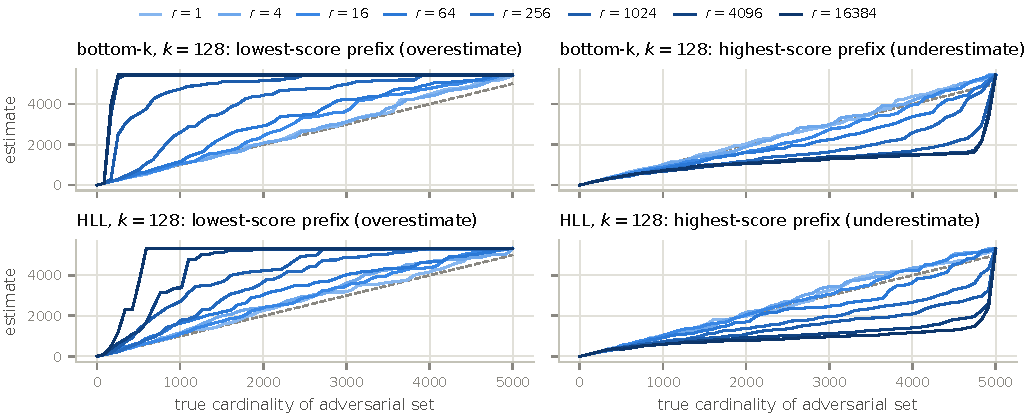
\includegraphics[width=\textwidth]{figures/fig_e2_k128}
\caption{Attack strength vs.\ number of queries $r$ ($k=128$, $n=5000$; cf.\ Figures~1--2 of~\cite{ahmadian2024}). Each curve adds keys in increasing (top-left, bottom-left) or decreasing (right) order of their average score after $r$ queries; the dashed line is a perfect estimate.}
\label{fig:e2}
\end{figure*}

\begin{figure*}[t]
\centering
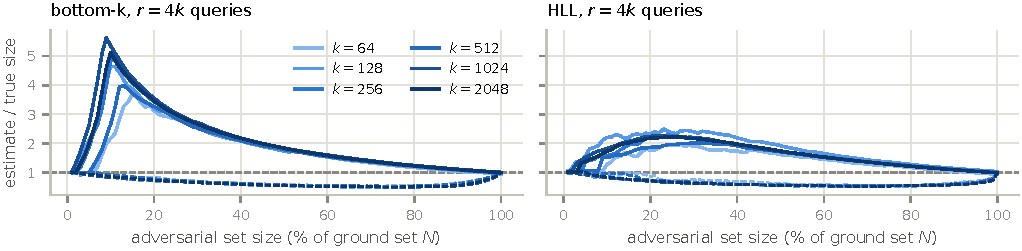
\includegraphics[width=\textwidth]{figures/fig_e3_sizes}
\caption{Attack strength vs.\ sketch size with $r=4k$ queries and $n=10\cdot 10^{\lceil\log_{10}k\rceil}$ (cf.\ Figure~3 of~\cite{ahmadian2024}). Solid: lowest-score prefix; dashed: highest-score prefix. Mean of 3 seeds.}
\label{fig:e3}
\end{figure*}

\subsection{Attacks on any estimator (Problem 3)}

Algorithm~1 relies on the estimator reporting a sufficient statistic. A cleverer query-response (QR) algorithm could, for instance, return $n/2$ on every query: the queries of Algorithm~1 all have size close to $n/2$, so this answer is correct and leaks nothing. To show that the \emph{sketch structure itself} is vulnerable, \cite{ahmadian2024} consider a much stronger QR algorithm: it knows the attacker's query distribution and internal state, sees the identities of the keys that determine the sketch, and only has to solve the \emph{soft threshold} problem (is $|U|\le A$ or $|U|\ge 2A$?) correctly with probability $1-\delta$ over the query distribution. The attacker varies the sampling rate $q$ of its queries so that the size of $U$ is unpredictable.

\emph{Several rounds are necessary} (Lemma~6.5). Against a single batch of $r$ queries, the QR algorithm can answer every query from one fixed sub-sketch of only $k'=O(\log(r/\delta))$ components, e.g.\ $k'$ of the $k$ hash functions, because the non-adaptive union bound applies to it. The answers then reveal nothing about the other $k-k'$ components, so forcing the QR algorithm to expose the whole sketch in one batch requires $r$ exponential in $k$.

\emph{Single batch vs.\ symmetric QR} (Algorithm~3, Theorem~7.1). If the QR map must treat sketch components symmetrically and be monotone, a single batch of $\tilde O(k^2)$ queries suffices. Here the score gap between a low-priority key and a transparent key is only $\tilde\Omega(1/k)$ per query (Lemma~7.3), while the per-query noise is constant, so $r=\tilde O(k^2)$ queries are needed for a Chernoff bound to separate them. The keys with score above the median plus $\tilde\Omega(r/k)$ form a mask $M$ with $S_\rho(M)=S_\rho(N)$.

\emph{Adaptive attack on any correct QR} (Algorithm~4, Theorem~8.1). The attacker adds a key to the mask $M$ as soon as its score separates from the median, and from then on queries $M\cup U$. As $M$ absorbs low-priority keys, the effective sketch of the remaining keys shrinks. Either the QR algorithm fails, or after $r=\tilde O(k^2/\alpha^2)$ queries the mask contains all low-priority keys while $|M|<\alpha n$. Then $S_\rho(M\cup U)\approx S_\rho(M)$ for any $U$ and no estimator can recover $|U|$. This quadratic bound matches the generic robustness upper bound of Hassidim et al.~\cite{hassidim2020}, so it is tight up to log factors.

%=========================================================================
\section{Experiments}

\paragraph{Setup.}
We implemented bottom-$k$ and HLL in Python/NumPy.\footnote{Code, data and figures: \url{https://github.com/Juno9170/COMP-4801-Project-Report}} Keys are integers, each hashed once with a fixed, seeded 64-bit hash (splitmix64). A query is stored as one true/false flag per key of $N$, and its sketch is computed from the precomputed hash values of the flagged keys. Only hash values matter, so this is equivalent to hashing strings as in~\cite{ahmadian2024}. Our HLL uses $k=2^p$ registers and the estimator of~\cite{flajolet2007} with linear counting for small sets. The paper uses an open-source HLL++ implementation; in the regime $n\gg k$ that we study, HLL++ runs in dense mode and gives the same estimates as HLL, except for its small-range bias correction. Because HLL needs $k$ to be a power of two, we use $k=128$ and $512$ where the paper uses $104$ and $416$. All runs use fixed seeds.

\paragraph{Non-adaptive accuracy.}
For random sets of $10^4$ keys (200 trials, fresh keys each time), the NRMSE of both sketches tracks $1/\sqrt{k}$ for $k=64,\dots,2048$ (e.g.\ $0.125, 0.043, 0.020$ for bottom-$k$ and $0.125, 0.046, 0.021$ for HLL at $k=64, 512, 2048$). Bottom-$k$ is within 4\% of $1/\sqrt{k}$, and HLL is within 12\% of it, close to its theoretical $1.04/\sqrt{k}$. Errors caused by the attack are therefore far outside the $\pm 3/\sqrt{k}$ range.

\paragraph{Attack strength vs.\ number of queries.}
Figure~\ref{fig:e2} repeats the experiment of~\cite[Figs.~1--2]{ahmadian2024} with $k=128$ and a ground set of $n=5000$ keys. With $r=1$ the curves follow the diagonal, which is the non-adaptive regime. Even here the maximum over 60 prefixes deviates by up to $1.18\times$, and this is the noise floor for the numbers below. As $r$ grows, the lowest-score prefixes are overestimated more and more. For HLL the worst ratio is $2.9\times$ at $r=1024$, $4.3\times$ at $r=4096$ and $8.9\times$ at $r=16384$, where a set of about 600 keys is estimated at about 5300, the size of all of $N$. Bottom-$k$ breaks faster: at $r=4096$ a prefix of about 250 keys already has the full sketch of $N$ ($20\times$ overestimate). The highest-score prefixes are underestimated to $0.29\times$ (HLL) and $0.34\times$ (bottom-$k$). With $k=512$ (not shown) the same effects need roughly four times as many queries: e.g., HLL at $r=4096$ reaches $1.9\times$ and $0.52\times$, compared with $2.9\times$ and $0.52\times$ for $k=128$ at $r=1024$. This is the linear dependence on $k$ that the theory predicts.

\paragraph{Attack strength vs.\ sketch size.}
Figure~\ref{fig:e3} and Table~\ref{tab:e3} repeat~\cite[Fig.~3]{ahmadian2024}: $r=4k$ queries for $k=2^6,\dots,2^{11}$. The key observation is that the curves for different $k$ nearly coincide. With a query budget proportional to $k$, the attack does equally well at every sketch size, which is direct empirical evidence that $O(k)$ queries suffice. For HLL, the worst lowest-score prefix is overestimated by $2.0$--$2.7\times$ (mean $2.3\times$ over the six values of $k$), and the worst highest-score prefix is underestimated to $0.51$--$0.54\times$.

\begin{table}[t]
\centering\small
\begin{tabular}{rrcccc}
\toprule
 & & \multicolumn{2}{c}{bottom-$k$} & \multicolumn{2}{c}{HLL}\\
$k$ & $n$ & over & under & over & under\\
\midrule
64   & $10^3$ & 3.76 & 0.51 & 2.04 & 0.53\\
128  & $10^4$ & 4.66 & 0.49 & 2.72 & 0.51\\
256  & $10^4$ & 4.95 & 0.49 & 2.33 & 0.54\\
512  & $10^4$ & 4.04 & 0.53 & 2.06 & 0.54\\
1024 & $10^5$ & 5.63 & 0.50 & 2.29 & 0.53\\
2048 & $10^5$ & 5.13 & 0.50 & 2.24 & 0.53\\
\bottomrule
\end{tabular}
\caption{Worst estimate/true ratio over prefixes, $r=4k$ (mean of 3 seeds). ``Over'': lowest-score prefix; ``under'': highest-score prefix.}
\label{tab:e3}
\end{table}

\paragraph{Comparison with the paper.}
Ahmadian and Cohen report that with $4k$ queries HLL++ overestimates or underestimates by about 40\%, and their Figure~3 peaks at a ratio of roughly $1.6$--$1.8$ at 20--40\% of the ground set. Our HLL curves have the same shape, with the peak at 21--38\% of $N$, and the same independence from $k$, but are somewhat stronger (peaks $2.0$--$2.7$). We did not isolate the cause. Plausible ones are differences between our HLL and their HLL++ implementation (hash function, bias correction), the slightly different $k$ values, and averaging over seeds. Either way, the paper's central empirical claim is reproduced: a single batch of $4k$ non-adaptive queries suffices for errors of 40\% or more at every sketch size we tested.

\paragraph{Bottom-$k$ vs.\ HLL.}
Bottom-$k$, the sketch Theorem~4.1 is actually about, is about twice as vulnerable: with $r=4k$, prefixes of about 10\% of $N$ are overestimated by $3.8$--$5.6\times$ (mean $4.7\times$), i.e.\ estimated at about $0.5n$, in line with the theorem's $\Theta(n)$. Our explanation is discretization. HLL registers store a rounded rank, so the maximum in a register is often shared by several keys of its bucket. Removing one of them then does not change the estimate, which weakens the per-query signal about that key. Bottom-$k$ keeps full-precision values, and every one of its $k$ keys affects the estimate. This agrees with the remark in~\cite{ahmadian2024} that results are stronger when the full-precision representation is available.

\begin{figure}[t]
\centering
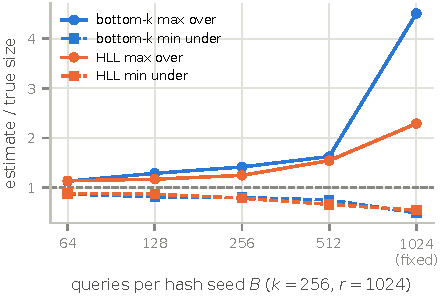
\includegraphics[width=\columnwidth]{figures/fig_e4_mitigation}
\caption{Mitigation: the system re-draws its hash seed every $B$ queries ($k=256$, $n=10^4$, $r=4k$, 3 seeds); the adversarial sets are evaluated under the final seed.}
\label{fig:e4}
\end{figure}

\paragraph{Mitigation.}
The simplest defense is to stop reusing randomness: the system draws a fresh hash seed every $B$ queries. The attacker keeps accumulating scores, and we evaluate its adversarial sets under the seed in use at the end (Figure~\ref{fig:e4}). With $B\le k/2$ the attack is reduced to the noise floor ($\le 1.3\times$ over, $\ge 0.81\times$ under). Even $B=2k$ cuts the HLL overestimate from $2.3\times$ to $1.5\times$, because only the last $B$ queries carry information about the current seed. The price is composability. Sketches built under different seeds cannot be merged, so the system must either rebuild stored sketches from raw data, defeating the purpose of sketching, or keep one sketch per epoch, paying the linear-in-$r$ space of the generic ``fresh copy'' approach~\cite{ahmadian2024}.

%=========================================================================
\section{Conclusions}

Cardinality sketches are accurate for any \emph{fixed} query, but their guarantees rest on the query being independent of the hash randomness, which composability forces to be shared and reused. Ahmadian and Cohen show that this assumption can be exploited cheaply: $O(k)$ non-adaptive random queries and an averaging step expose the low-priority keys of the standard estimators, and $\tilde O(k^2)$ adaptive queries defeat any estimator. Our implementation confirms that the linear attack is practical and works with small constants. With $r=4k$ queries, for every $k$ from 64 to 2048, HLL is overestimated by $2.3\times$ on average and underestimated by about half, and bottom-$k$ is overestimated by $4.7\times$ on average. Re-drawing the randomness often removes the effect, but only by giving up the mergeability that makes sketches useful.

\paragraph{What I learned.}
The most useful lesson was where the probabilistic guarantee lives. ``With high probability over $\rho$, for every query'' and ``for every query, with high probability over $\rho$'' are different statements, and the union bound only gives the second for a set of queries fixed in advance. The same gap appeared with Bloom filters and with oblivious versus adaptive adversaries in online learning. Implementing the attack also made the signal-to-noise argument concrete: each query gives a $1/\sqrt{k}$-strength signal about each key, and averaging over $\Theta(k)$ queries is exactly what makes it visible.

\paragraph{Future work.}
Cohen, Singhal and Stemmer~\cite{cohen2025} show that the quadratic barrier is not a limit for all workloads. With robust estimators they answer many more adaptive queries when no single key takes part in too many of them, which matches the suggestion in~\cite{ahmadian2024} to limit how often each key is queried. A natural next step is to implement such an estimator and Algorithm~4 and measure how the number of queries needed scales with $k$.

%---------------------------- Bibliography -------------------------------
\clearpage
\small
\bibliographystyle{abbrv}
\bibliography{refs}

\end{document}
